\documentclass[11pt,a4paper]{report}
\usepackage[textwidth=37em,vmargin=30mm]{geometry}
\usepackage{calc,xunicode,amsmath,amssymb,paralist,enumitem,tabu,booktabs,datetime2,xeCJK,xeCJKfntef,listings}
\usepackage{tocloft,fancyhdr,tcolorbox,xcolor,graphicx,eso-pic,xltxtra,xelatexemoji}

\newcommand{\envyear}[0]{2025}
\newcommand{\envdatestr}[0]{2025-05-08}
\newcommand{\envfinaldir}[0]{webdb/2025/20250508/final}

\usepackage[hidelinks]{hyperref}
\hypersetup{
    colorlinks=false,
    pdfpagemode=FullScreen,
    pdftitle={Web Digest - \envdatestr}
}

\setlength{\cftbeforechapskip}{10pt}
\renewcommand{\cftchapfont}{\rmfamily\bfseries\large\raggedright}
\setlength{\cftbeforesecskip}{2pt}
\renewcommand{\cftsecfont}{\sffamily\small\raggedright}

\setdefaultleftmargin{2em}{2em}{1em}{1em}{1em}{1em}

\usepackage{xeCJK,xeCJKfntef}
\xeCJKsetup{PunctStyle=plain,RubberPunctSkip=false,CJKglue=\strut\hskip 0pt plus 0.1em minus 0.05em,CJKecglue=\strut\hskip 0.22em plus 0.2em}
\XeTeXlinebreaklocale "zh"
\XeTeXlinebreakskip = 0pt


\setmainfont{Brygada 1918}
\setromanfont{Brygada 1918}
\setsansfont{IBM Plex Sans}
\setmonofont{JetBrains Mono NL}
\setCJKmainfont{Noto Serif CJK SC}
\setCJKromanfont{Noto Serif CJK SC}
\setCJKsansfont{Noto Sans CJK SC}
\setCJKmonofont{Noto Sans CJK SC}

\setlength{\parindent}{0pt}
\setlength{\parskip}{8pt}
\linespread{1.15}

\lstset{
	basicstyle=\ttfamily\footnotesize,
	numbersep=5pt,
	backgroundcolor=\color{black!5},
	showspaces=false,
	showstringspaces=false,
	showtabs=false,
	tabsize=2,
	captionpos=b,
	breaklines=true,
	breakatwhitespace=true,
	breakautoindent=true,
	linewidth=\textwidth
}






\newcommand{\coverpic}[2]{
    % argv: itemurl, authorname
    Cover photo by #2~~(\href{#1}{#1})
}
\newcommand{\makeheader}[0]{
    \begin{titlepage}
        % \newgeometry{hmargin=15mm,tmargin=21mm,bmargin=12mm}
        \begin{center}
            
            \rmfamily\scshape
            \fontspec{BaskervilleF}
            \fontspec{Old Standard}
            \fontsize{59pt}{70pt}\selectfont
            WEB\hfill DIGEST
            
            \vfill
            % \vskip 30pt
            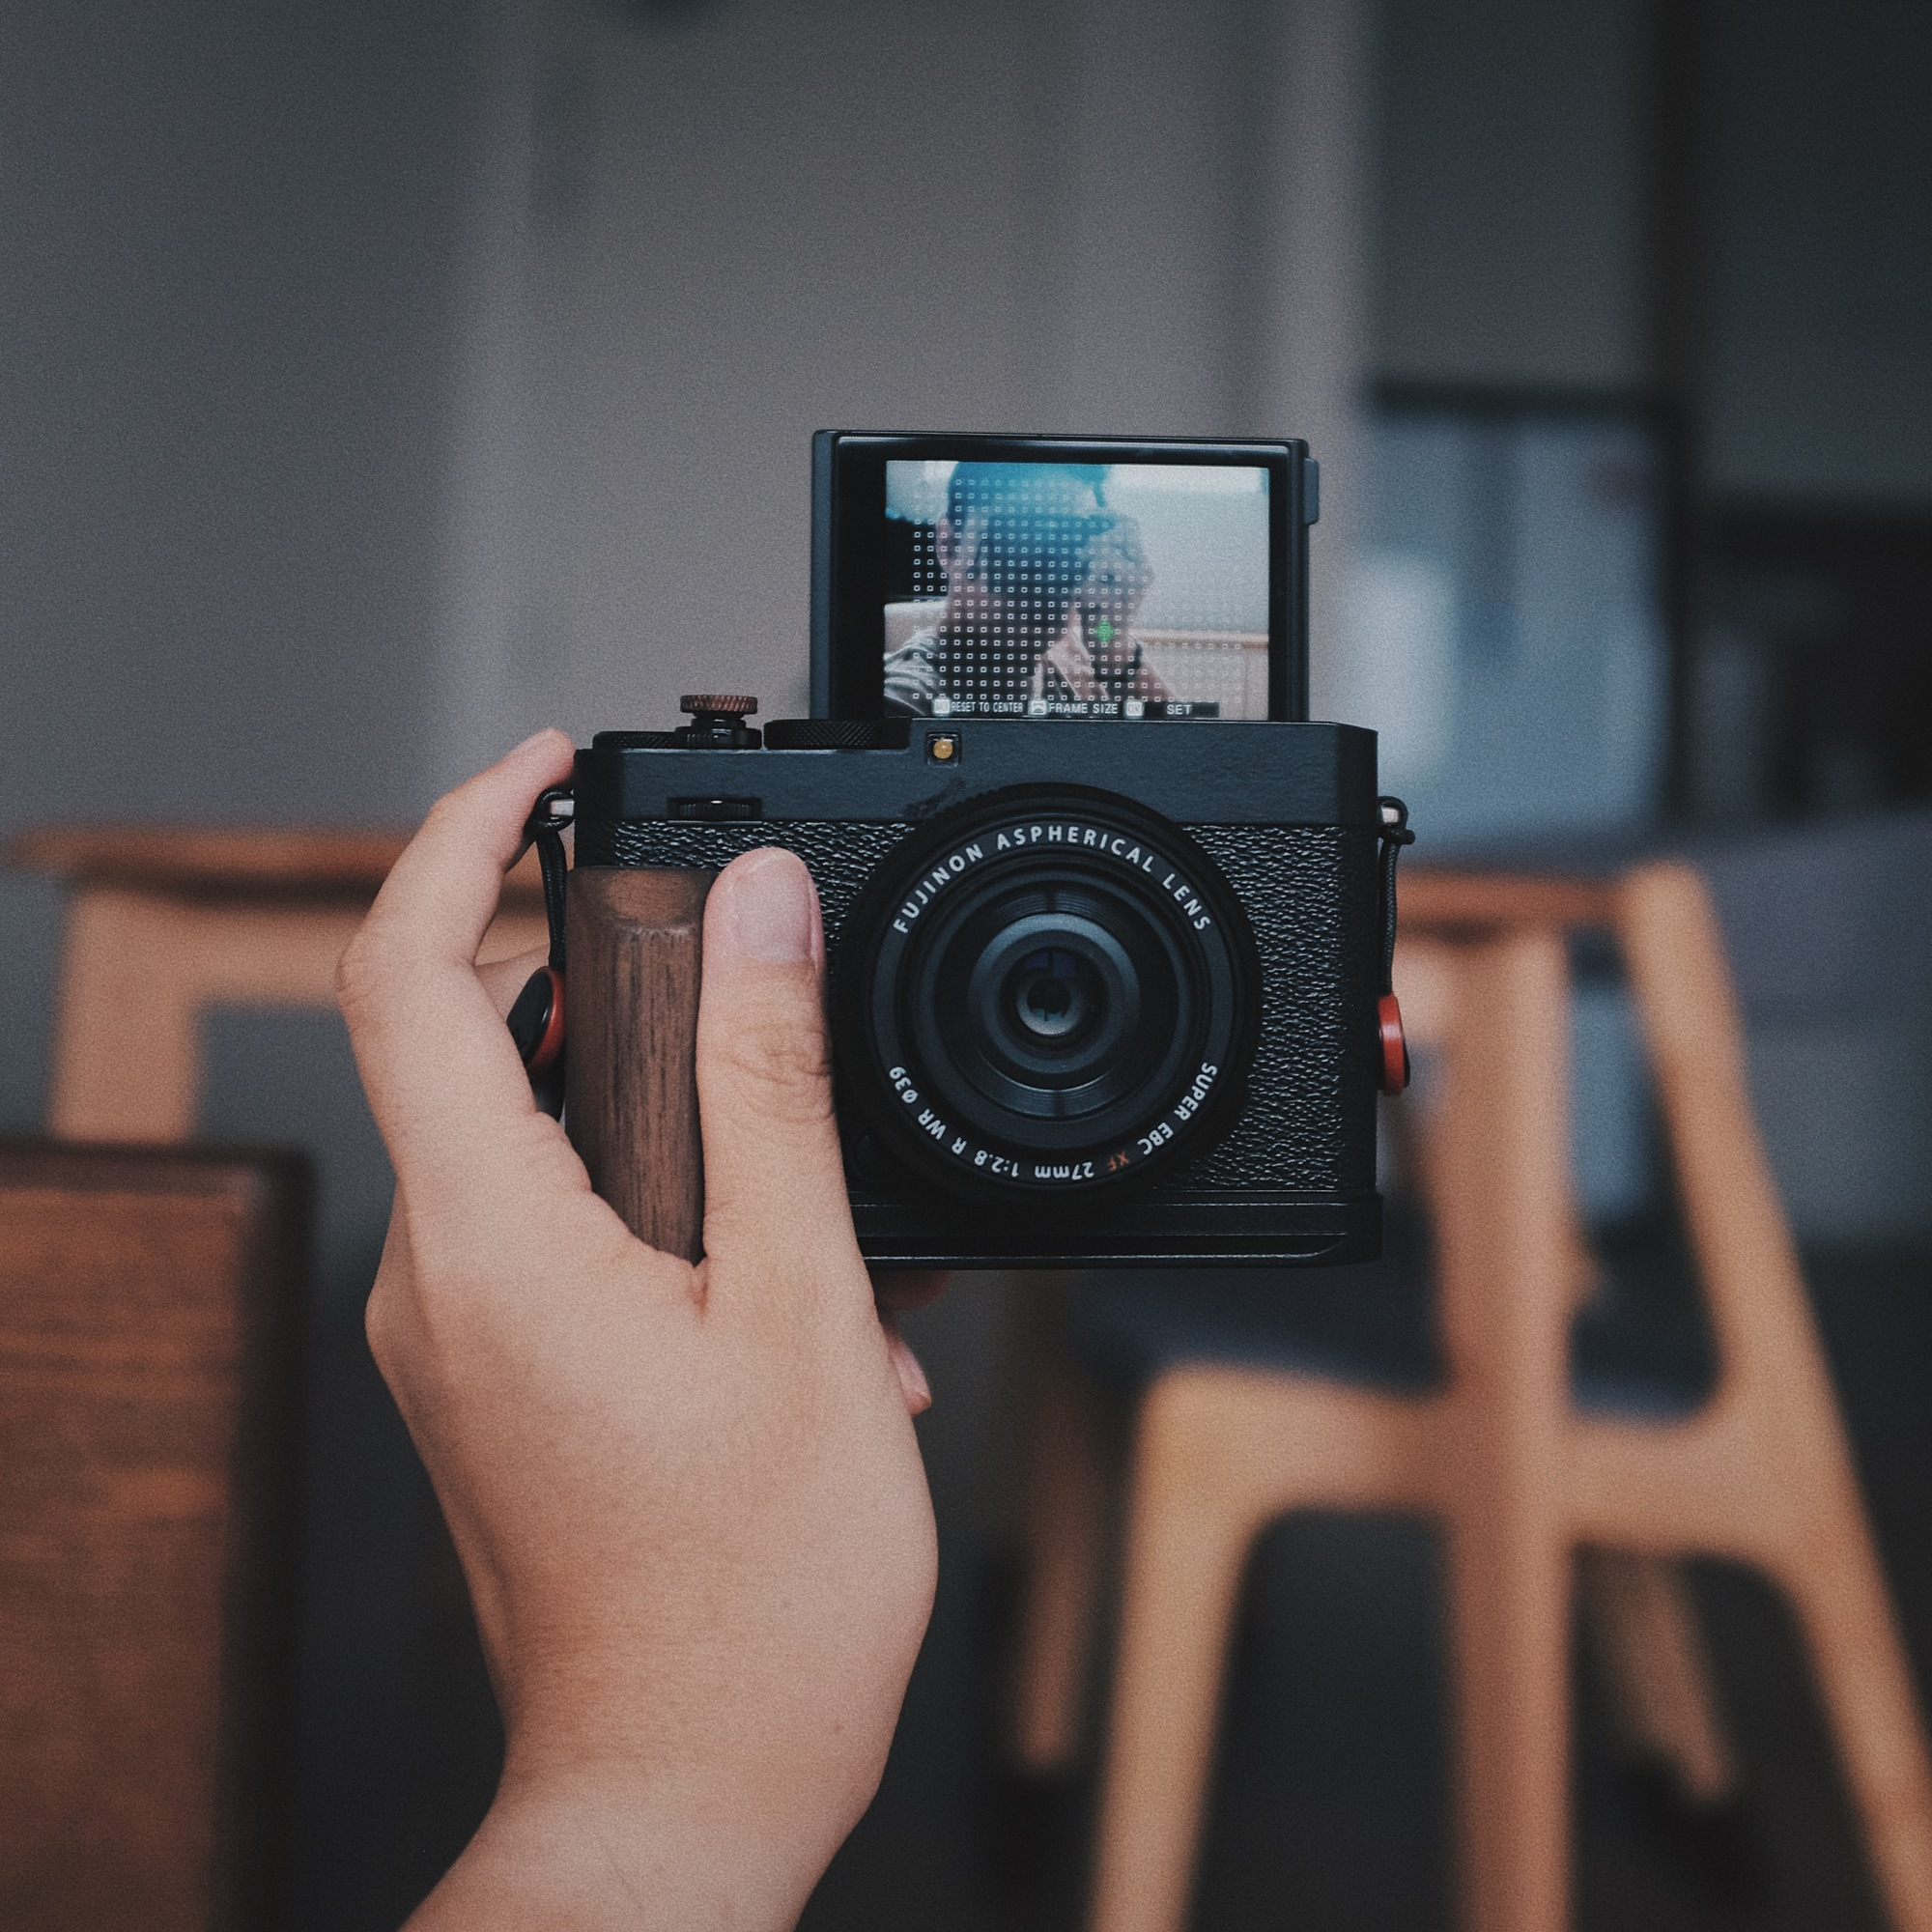
\includegraphics[width=\linewidth]{\envfinaldir/coverpic-prod.jpg}\par
            % \vskip 30pt
            \vfill

            \normalsize\rmfamily\scshape
            \copyright{} The Web Digest Project \hfill\large \envdatestr
        \end{center}
    \end{titlepage}
    % \restoregeometry
}
\newcommand{\simplehref}[1]{%
    \textcolor{blue!80!green}{\href{#1}{#1}}%
}
\renewcommand{\contentsname}{\center\Huge\sffamily\bfseries Contents\par\vskip 20pt}
\newcounter{ipartcounter}
\setcounter{ipartcounter}{0}
\newcommand{\ipart}[1]{
    % \vskip 20pt
    \clearpage
    \stepcounter{ipartcounter}
    \phantomsection
    \addcontentsline{toc}{chapter}{#1}
    % \begin{center}
    %     \Huge
    %     \sffamily\bfseries
    %     #1
    % \end{center}
    % \vskip 20pt plus 7pt
}
\newcounter{ichaptercounter}
\setcounter{ichaptercounter}{0}
\newcommand{\ichapter}[1]{
    % \vskip 20pt
    \clearpage
    \stepcounter{ichaptercounter}
    \phantomsection
    \addcontentsline{toc}{section}{\numberline{\arabic{ichaptercounter}}#1}
    \begin{center}
        \Huge
        \sffamily\bfseries
        #1
    \end{center}
    \vskip 20pt plus 7pt
}
\newcommand{\entrytitlefont}[1]{\subsection*{\raggedright\Large\sffamily\bfseries#1}}
\newcommand{\entryitemGeneric}[2]{
    % argv: title, url
    \parbox{\linewidth}{
        \entrytitlefont{#1}\par\vskip 5pt
        \footnotesize\ttfamily\mdseries
        \simplehref{#2}
    }\vskip 11pt plus 11pt minus 1pt
}
\newcommand{\entryitemGithub}[3]{
    % argv: title, url, desc
    \parbox{\linewidth}{
        \entrytitlefont{#1}\par\vskip 5pt
        \footnotesize\ttfamily\mdseries
        \simplehref{#2}\par\vskip 5pt
        \small\rmfamily\mdseries#3
    }\vskip 11pt plus 11pt minus 1pt
}
\newcommand{\entryitemAp}[3]{
    % argv: title, url, desc
    \parbox{\linewidth}{
        \entrytitlefont{#1}\par\vskip 5pt
        \footnotesize\ttfamily\mdseries
        \simplehref{#2}\par\vskip 5pt
        \small\rmfamily\mdseries#3
    }\vskip 11pt plus 11pt minus 1pt
}
\newcommand{\entryitemHackernews}[3]{
    % argv: title, hnurl, rawurl
    % \parbox{\linewidth}{
    %     \entrytitlefont{#1}\par\vskip 5pt
    %     \footnotesize\ttfamily\mdseries
    %     \simplehref{#3}\par
    %     \textcolor{black!50}{\href{#2}{#2}}
    % }\vskip 11pt plus 11pt minus 1pt
    \begin{minipage}{\linewidth}
            \entrytitlefont{#1}\par\vskip 5pt
            \footnotesize\ttfamily\mdseries
            \simplehref{#3}\par
            \textcolor{black!50}{\href{#2}{#2}}
    \end{minipage}\par\vskip 11pt plus 11pt minus 1pt
}







\begin{document}

\makeheader

\tableofcontents\clearpage




\ipart{Developers}
\ichapter{Hacker News}
\entryitemTwoLinks{Introducing Web Search on the Anthropic API}{https://news.ycombinator.com/item?id=43920188}{https://www.anthropic.com/news/web-search-api}

\entryitemTwoLinks{Open source Google Analytics replacement}{https://news.ycombinator.com/item?id=43918620}{https://github.com/rybbit-io/rybbit}

\entryitemTwoLinks{Three Chapters at Cloudflare: Programmer to CTO to Board of Directors}{https://news.ycombinator.com/item?id=43918600}{https://blog.cloudflare.com/en-us/three-chapters-at-cloudflare-programmer-to-cto-to-board-of-directors/}

\entryitemTwoLinks{Ty: A fast Python type checker and language server}{https://news.ycombinator.com/item?id=43918484}{https://github.com/astral-sh/ty}

\entryitemTwoLinks{Getting Older Isn't What You Think}{https://news.ycombinator.com/item?id=43917855}{https://www.katycowan.co.uk/blog/getting-old}

\entryitemTwoLinks{Create and edit images with Gemini 2.0 in preview}{https://news.ycombinator.com/item?id=43917461}{https://developers.googleblog.com/en/generate-images-gemini-2-0-flash-preview/}

\entryitemTwoLinks{Show HN: eInk optimized manga with Kindle Comic Converter (+Kobo/ReMarkable)}{https://news.ycombinator.com/item?id=43916956}{https://github.com/ciromattia/kcc}

\entryitemTwoLinks{Waiting for Postgres 18: Accelerating Disk Reads with Asynchronous I/O}{https://news.ycombinator.com/item?id=43916577}{https://pganalyze.com/blog/postgres-18-async-io}

\entryitemTwoLinks{Mistral ships le chat – enterprise AI assistant that can run on prem}{https://news.ycombinator.com/item?id=43916098}{https://mistral.ai/news/le-chat-enterprise}

\entryitemTwoLinks{Unity's Open-Source Double Standard: the ban of VLC}{https://news.ycombinator.com/item?id=43914832}{https://mfkl.github.io/2024/01/10/unity-double-oss-standards.html}

\entryitemTwoLinks{CLion Is Now Free for Non-Commercial Use}{https://news.ycombinator.com/item?id=43914705}{https://blog.jetbrains.com/clion/2025/05/clion-is-now-free-for-non-commercial-use/}

\entryitemTwoLinks{My quest to make motorcycle riding that tad bit safer}{https://news.ycombinator.com/item?id=43914235}{https://gill.net.in/posts/my-quest-to-make-motorcycle-riding-safer/}

\entryitemTwoLinks{So Much Blood}{https://news.ycombinator.com/item?id=43913751}{https://dynomight.net/blood/}

\entryitemTwoLinks{Zed: High-performance AI Code Editor}{https://news.ycombinator.com/item?id=43912844}{https://zed.dev/blog/fastest-ai-code-editor}

\entryitemTwoLinks{EPA Plans to Shut Down the Energy Star Program}{https://news.ycombinator.com/item?id=43911252}{https://www.nytimes.com/2025/05/06/climate/epa-energy-star-eliminated.html}

\entryitemTwoLinks{Jury orders NSO to pay \$167M for hacking WhatsApp users}{https://news.ycombinator.com/item?id=43911167}{https://arstechnica.com/security/2025/05/jury-orders-nso-to-pay-167-million-for-hacking-whatsapp-users/}

\entryitemTwoLinks{FTC bans hidden fees for live events and short-term rentals, effective May 12}{https://news.ycombinator.com/item?id=43910794}{https://techcrunch.com/2025/05/05/ftc-bans-hidden-fees-for-live-events-and-short-term-rentals-effective-may-12/}

\entryitemTwoLinks{Bloat is still software's biggest vulnerability (2024)}{https://news.ycombinator.com/item?id=43910745}{https://spectrum.ieee.org/lean-software-development}

\entryitemTwoLinks{The DEA is now abandoning body cameras}{https://news.ycombinator.com/item?id=43910720}{https://www.propublica.org/article/drug-enforcement-administration-ends-body-camera-program-trump}

\entryitemTwoLinks{Alignment is not free: How model upgrades can silence your confidence signals}{https://news.ycombinator.com/item?id=43910685}{https://www.variance.co/post/alignment-is-not-free-how-a-model-silenced-our-confidence-signals}\ichapter{Phoronix}
\entryitemGeneric{\hskip 0pt{}Intel Teases New Arc Pro Graphics Cards Ahead Of Computex}{https://www.phoronix.com/news/Intel-Arc-Pro-Taipei}

\entryitemGeneric{\hskip 0pt{}New GNOME Executive Director Named: Steven Deobald}{https://www.phoronix.com/news/GNOME-Executive-Steven-Deobald}

\entryitemGeneric{\hskip 0pt{}Mesa 25.1 Released With Many Open-Source Vulkan Driver Improvements}{https://www.phoronix.com/news/Mesa-25.1-Released}

\entryitemGeneric{\hskip 0pt{}Fwupd 2.0.9 Released With Firmware Updating Support For Intel Arc Battlemage}{https://www.phoronix.com/news/Fwupd-2.0.9-Released}

\entryitemGeneric{\hskip 0pt{}Raspberry Pi OS Updated With More Wayland Work, Likely The Last Based On Debian 12}{https://www.phoronix.com/news/Raspberry-Pi-OS-May-2025}

\entryitemGeneric{\hskip 0pt{}AMD Strix Point \& Intel Lunar Lake: Windows 11 vs. Ubuntu 25.04 Linux Performance}{https://www.phoronix.com/review/lunarlake-windows11-ubuntu2504}

\entryitemGeneric{\hskip 0pt{}Loongson To Up Linux Kernel Limit To 2,048 LoongArch CPU Cores}{https://www.phoronix.com/news/LoongArch-Linux-2048-CPU-Cores}

\entryitemGeneric{\hskip 0pt{}Linux 6.16 To Introduce Block Write Streams For NVMe Flexible Data Placement "FDP"}{https://www.phoronix.com/news/NVMe-FDP-Block-Linux-6.16}

\entryitemGeneric{\hskip 0pt{}Intel Introducing QAT "GEN6" Driver To The Linux Kernel}{https://www.phoronix.com/news/Intel-QAT-GEN6-Linux-Driver}\ichapter{Dribbble}
\entryitemGeneric{\hskip 0pt{}Modernizing the Website of a Shopify Email Customizer}{https://dribbble.com/shots/25993532-Modernizing-the-Website-of-a-Shopify-Email-Customizer}

\entryitemGeneric{\hskip 0pt{}Travel Startup Branding for Holidu: visual identity brand design}{https://dribbble.com/shots/25941954-Travel-Startup-Branding-for-Holidu-visual-identity-brand-design}

\entryitemGeneric{\hskip 0pt{}verif.ai}{https://dribbble.com/shots/25993296-verif-ai}

\entryitemGeneric{\hskip 0pt{}AI Security}{https://dribbble.com/shots/25987123-AI-Security}

\entryitemGeneric{\hskip 0pt{}Fiyah > Hot Sauces Line}{https://dribbble.com/shots/25989187-Fiyah-Hot-Sauces-Line}

\entryitemGeneric{\hskip 0pt{}Just a Hippo}{https://dribbble.com/shots/25988582-Just-a-Hippo}

\entryitemGeneric{\hskip 0pt{}Crypto Portfolio Tracker App}{https://dribbble.com/shots/25988631-Crypto-Portfolio-Tracker-App}

\entryitemGeneric{\hskip 0pt{}Unused Logo Concept for FinAi}{https://dribbble.com/shots/25989542-Unused-Logo-Concept-for-FinAi}

\entryitemGeneric{\hskip 0pt{}Mobile App Work Session Tracker}{https://dribbble.com/shots/25975579-Mobile-App-Work-Session-Tracker}

\entryitemGeneric{\hskip 0pt{}Tees High™ Monogram}{https://dribbble.com/shots/25990424-Tees-High-Monogram}

\entryitemGeneric{\hskip 0pt{}Quartz Wordmark Logo}{https://dribbble.com/shots/25985137-Quartz-Wordmark-Logo}

\entryitemGeneric{\hskip 0pt{}Fianance Landing Page}{https://dribbble.com/shots/25980595-Fianance-Landing-Page}

\entryitemGeneric{\hskip 0pt{}Heliara}{https://dribbble.com/shots/25983106-Heliara}

\entryitemGeneric{\hskip 0pt{}UI/UX Design for AURA — your personal AI assistant}{https://dribbble.com/shots/25982086-UI-UX-Design-for-AURA-your-personal-AI-assistant}

\entryitemGeneric{\hskip 0pt{}Envisioning the future}{https://dribbble.com/shots/25985271-Envisioning-the-future}

\entryitemGeneric{\hskip 0pt{}GOCCO Wordmark}{https://dribbble.com/shots/25984476-GOCCO-Wordmark}

\entryitemGeneric{\hskip 0pt{}Lume}{https://dribbble.com/shots/25978139-Lume}

\entryitemGeneric{\hskip 0pt{}Illustration}{https://dribbble.com/shots/25975830-Illustration}

\entryitemGeneric{\hskip 0pt{}Medical Landing Page Design}{https://dribbble.com/shots/25971117-Medical-Landing-Page-Design}

\entryitemGeneric{\hskip 0pt{}Onboarding illustrations set on UI8}{https://dribbble.com/shots/25973282-Onboarding-illustrations-set-on-UI8}

\entryitemGeneric{\hskip 0pt{}Mozambique}{https://dribbble.com/shots/25970792-Mozambique}

\entryitemGeneric{\hskip 0pt{}Order details modal calendar dashboard}{https://dribbble.com/shots/25966379-Order-details-modal-calendar-dashboard}

\entryitemGeneric{\hskip 0pt{}W Letter Logo Concept}{https://dribbble.com/shots/25970255-W-Letter-Logo-Concept}

\entryitemGeneric{\hskip 0pt{}Phantom apple watch}{https://dribbble.com/shots/25967884-Phantom-apple-watch}


\ipart{Developers~~~~(zh-Hans)}
\ichapter{Solidot}
\entryitemGeneric{\hskip 0pt{}微软对因绩效不佳而解雇的员工实施两年禁聘令}{https://www.solidot.org/story?sid=81223}

\entryitemGeneric{\hskip 0pt{}特朗普政府官员使用的修改版 Signal 暂停服务}{https://www.solidot.org/story?sid=81222}

\entryitemGeneric{\hskip 0pt{}Mr. Deepfakes 永久关闭}{https://www.solidot.org/story?sid=81221}

\entryitemGeneric{\hskip 0pt{}古代诗歌揭示江豚的历史分布}{https://www.solidot.org/story?sid=81220}

\entryitemGeneric{\hskip 0pt{}阿联酋将为中小学生开设 AI 课程}{https://www.solidot.org/story?sid=81219}

\entryitemGeneric{\hskip 0pt{}OpenAI 宣布其非盈利实体将保留控股权}{https://www.solidot.org/story?sid=81218}

\entryitemGeneric{\hskip 0pt{}有心理健康问题的青少年更可能长时间沉迷社媒}{https://www.solidot.org/story?sid=81217}

\entryitemGeneric{\hskip 0pt{}微软正式关闭 Skype}{https://www.solidot.org/story?sid=81216}

\entryitemGeneric{\hskip 0pt{}现代汽车在其美国工厂部署 Atlas 机器人}{https://www.solidot.org/story?sid=81215}

\entryitemGeneric{\hskip 0pt{}Half-Life 3 可能年内宣布}{https://www.solidot.org/story?sid=81214}

\entryitemGeneric{\hskip 0pt{}洗衣机难以真正消毒}{https://www.solidot.org/story?sid=81213}

\entryitemGeneric{\hskip 0pt{}日本 15 岁以下儿童首次跌破 1400 万}{https://www.solidot.org/story?sid=81212}

\entryitemGeneric{\hskip 0pt{}特朗普政府大幅削减 NASA 预算,将重心转移到火星}{https://www.solidot.org/story?sid=81211}

\entryitemGeneric{\hskip 0pt{}北美鸟类加快消减 }{https://www.solidot.org/story?sid=81210}

\entryitemGeneric{\hskip 0pt{}Threads 用户数突破 3.5 亿}{https://www.solidot.org/story?sid=81209}

\entryitemGeneric{\hskip 0pt{}Mozilla 高管称没有 Google 的默认搜索交易它会倒闭}{https://www.solidot.org/story?sid=81208}\ichapter{V2EX}
\entryitemGeneric{\hskip 0pt{}[问与答] 购买手机求推荐}{https://www.v2ex.com/t/1130303}

\entryitemGeneric{\hskip 0pt{}[macOS] arc 的 ai 助手在使用分流规则时不能使用, 报 "Sorry, I encountered an error", 解决}{https://www.v2ex.com/t/1130302}

\entryitemGeneric{\hskip 0pt{}[职场话题] 遇到奇葩同事,工作上`效率 -99\%'+ 身边`生化武器',怎么应对?}{https://www.v2ex.com/t/1130301}

\entryitemGeneric{\hskip 0pt{}[职场话题] 感觉快活不下去了}{https://www.v2ex.com/t/1130300}

\entryitemGeneric{\hskip 0pt{}[问与答] 提示「无效的 store」,是否是账户封禁预告?}{https://www.v2ex.com/t/1130299}

\entryitemGeneric{\hskip 0pt{}[奇思妙想] 鉴于 gitee 悬赏功能将下线,打算在 github 开个悬赏窗口}{https://www.v2ex.com/t/1130298}

\entryitemGeneric{\hskip 0pt{}[macOS] 圈 x 更新了, 并且还涨价了 😂}{https://www.v2ex.com/t/1130297}

\entryitemGeneric{\hskip 0pt{}[随想] 记一次实锤手机监听事件}{https://www.v2ex.com/t/1130294}

\entryitemGeneric{\hskip 0pt{}[问与答] iPad pro2018 屏幕咨询}{https://www.v2ex.com/t/1130293}

\entryitemGeneric{\hskip 0pt{}[iPhone] 最新系统解决第三方 app 获取手机空间不准的问题了吗?}{https://www.v2ex.com/t/1130291}

\entryitemGeneric{\hskip 0pt{}[推广] 5000 本计算机编程电子书 PDF 分享}{https://www.v2ex.com/t/1130290}

\entryitemGeneric{\hskip 0pt{}[Apple] L 口的手机和 C 口的耳机,有没有什么办法可以少带一根充电器,求传授经验}{https://www.v2ex.com/t/1130289}

\entryitemGeneric{\hskip 0pt{}[程序员] 我是如何一步步的错误解决问题}{https://www.v2ex.com/t/1130288}

\entryitemGeneric{\hskip 0pt{}[问与答] Linux 上 fcitx5 跟 keyd 之间好像有兼容性问题}{https://www.v2ex.com/t/1130287}

\entryitemGeneric{\hskip 0pt{}[问与答] 从你身边来看,有多少比例的人躲过了此轮地产泡沫破灭的周期?}{https://www.v2ex.com/t/1130284}

\entryitemGeneric{\hskip 0pt{}[分享创造] [小玩具] Dog Name Checker - 给你的毛孩子找个完美名字}{https://www.v2ex.com/t/1130283}

\entryitemGeneric{\hskip 0pt{}[程序员] augment 真的涨价了}{https://www.v2ex.com/t/1130282}

\entryitemGeneric{\hskip 0pt{}[问与答] 好消息就在刚刚 CLion 对非商业用途免费了}{https://www.v2ex.com/t/1130281}

\entryitemGeneric{\hskip 0pt{}[分享创造] 助力播客发现和传播,准备做个中文播客发现 MCP 服务,怎么样}{https://www.v2ex.com/t/1130279}

\entryitemGeneric{\hskip 0pt{}[投资] 由大多数人炒股亏钱想到的一个赚钱方法?}{https://www.v2ex.com/t/1130278}

\entryitemGeneric{\hskip 0pt{}[宽带症候群] 请问你们的电信测速达标吗}{https://www.v2ex.com/t/1130277}

\entryitemGeneric{\hskip 0pt{}[问与答] 兄弟们不看的书都是怎么保存的}{https://www.v2ex.com/t/1130276}

\entryitemGeneric{\hskip 0pt{}[macOS] m4 macbook air + 30W 充电器接电源状态下电池掉电?}{https://www.v2ex.com/t/1130274}

\entryitemGeneric{\hskip 0pt{}[程序员] 构造大模型微调数据集}{https://www.v2ex.com/t/1130273}

\entryitemGeneric{\hskip 0pt{}[OpenAI] 我想问一下,目前 ChatGPT 网页端还有降智的现象么?}{https://www.v2ex.com/t/1130272}

\entryitemGeneric{\hskip 0pt{}[职场话题] 10 年前端,想找一个副业}{https://www.v2ex.com/t/1130270}

\entryitemGeneric{\hskip 0pt{}[C++] CLion 提供非商业免费使用了}{https://www.v2ex.com/t/1130269}

\entryitemGeneric{\hskip 0pt{}[问与答] FastSpring 现在只有一种方案了么 5.9\%+\$0.95}{https://www.v2ex.com/t/1130267}

\entryitemGeneric{\hskip 0pt{}[分享创造] 如何兼得个人效率和兴趣活跃?}{https://www.v2ex.com/t/1130266}

\entryitemGeneric{\hskip 0pt{}[职场话题] 想辞职,是直接裸辞,还是问上司申请大礼包?}{https://www.v2ex.com/t/1130265}

\entryitemGeneric{\hskip 0pt{}[酷工作] Hot/New Jobs:[成都][腾讯]招聘 kubernetes/golang/容器网络 方向高级工程师}{https://www.v2ex.com/t/1130264}

\entryitemGeneric{\hskip 0pt{}[酷工作] 远程岗位:(AI 数据标注)产品经理, 5-7 万月薪}{https://www.v2ex.com/t/1130261}

\entryitemGeneric{\hskip 0pt{}[生活] 三十岁左右的你,正处于什么状态?}{https://www.v2ex.com/t/1130260}

\entryitemGeneric{\hskip 0pt{}[问与答] V 友们有没有新冠后开始对花粉过敏的}{https://www.v2ex.com/t/1130258}

\entryitemGeneric{\hskip 0pt{}[分享创造] 让 AI 写了一个批量克隆 GitLab 项目的脚本}{https://www.v2ex.com/t/1130257}

\entryitemGeneric{\hskip 0pt{}[职场话题] 晕,学士证的照片竟然丢了}{https://www.v2ex.com/t/1130256}

\entryitemGeneric{\hskip 0pt{}[问与答] 618 打算买电饭煲,大家有什么推荐的吗?}{https://www.v2ex.com/t/1130249}

\entryitemGeneric{\hskip 0pt{}[职场话题] 星沙农商行和长沙中烟工业选哪个?}{https://www.v2ex.com/t/1130247}

\entryitemGeneric{\hskip 0pt{}[问与答] 求指教 V 友们 2025 年了 刚发现我的夸克网盘还是 10g 还有办法免费扩容到 1T 么? 那种 1 年有效期那种}{https://www.v2ex.com/t/1130246}

\entryitemGeneric{\hskip 0pt{}[程序员] 如何部署属于自己的代码仓库呢?}{https://www.v2ex.com/t/1130245}

\entryitemGeneric{\hskip 0pt{}[问与答] 有无类似帆软的数据中台开源项目}{https://www.v2ex.com/t/1130244}

\entryitemGeneric{\hskip 0pt{}[生活] 手机真的不能只看处理器、像素,拉黑红米}{https://www.v2ex.com/t/1130242}

\entryitemGeneric{\hskip 0pt{}[程序员] nvidia docker + yolo 训练时最好把网络禁用掉}{https://www.v2ex.com/t/1130241}

\entryitemGeneric{\hskip 0pt{}[问与答] 土蜂蜜卖不掉}{https://www.v2ex.com/t/1130240}

\entryitemGeneric{\hskip 0pt{}[宽带症候群] 想搞个家庭机柜,各位有什么建议}{https://www.v2ex.com/t/1130239}

\entryitemGeneric{\hskip 0pt{}[Apple] 近期才遇到的 iPhone 镜像的 bug}{https://www.v2ex.com/t/1130237}

\entryitemGeneric{\hskip 0pt{}[长沙] 五一回长沙老家体验}{https://www.v2ex.com/t/1130236}

\entryitemGeneric{\hskip 0pt{}[程序员] 使用 ai 从零开始实现一个在线计算笔记本: NoteCalc}{https://www.v2ex.com/t/1130233}

\entryitemGeneric{\hskip 0pt{}[程序员] gitlab 不能通过 https 来 clone 只能 ssh,大家有遇到过吗}{https://www.v2ex.com/t/1130232}

\entryitemGeneric{\hskip 0pt{}[生活] 硬刚南山税务局,赢了}{https://www.v2ex.com/t/1130231}


\ipart{Generic News}
\ichapter{AP News}
\entryitemWithDescription{\hskip 0pt{}Utah Mammoth is the permanent name of the NHL team in Salt Lake City}{https://apnews.com/article/31aa2fa9d1cbb825ba5e0b61815e58de}{}

\entryitemWithDescription{\hskip 0pt{}An alligator kills a Florida woman after tipping over her canoe, investigators say}{https://apnews.com/article/f2a59ae2b4beba84fc6e2395b2a4552f}{}

\entryitemWithDescription{\hskip 0pt{}Actor Michael Pitt charged with sex abuse, assault of ex-girlfriend in New York}{https://apnews.com/article/539e638bc7ec90ee068374aa650d7d3a}{}

\entryitemWithDescription{\hskip 0pt{}Baby seal stabbed on Oregon coast prompts search for suspect}{https://apnews.com/article/3a7217b816dbc4cb1cce497e4cc568a0}{}

\entryitemWithDescription{\hskip 0pt{}The Steelers move on from George Pickens by trading mercurial receiver to Cowboys}{https://apnews.com/article/2fd4c79337748c82b66994180c6999aa}{}

\entryitemWithDescription{\hskip 0pt{}Disney parks thrive in second quarter and company adds 1.4 million new streaming subscribers}{https://apnews.com/article/12a484b389359d746c703898d71697c3}{}

\entryitemWithDescription{\hskip 0pt{}Smokey Robinson accused by former housekeepers of sexual assault and rape}{https://apnews.com/article/1512119eb018782fffad29d1d0358724}{}

\entryitemWithDescription{\hskip 0pt{}Two Belgian teenagers found with 5,000 ants in Kenya given \$7,700 fine or 1-year prison sentence}{https://apnews.com/article/50fc1a7141f515cc900f403ec93b06e5}{}

\entryitemWithDescription{\hskip 0pt{}Man arrested after ramming car into front gate of Jennifer Aniston's Los Angeles home}{https://apnews.com/article/22242e5a78afcb304b7d2d91bb4748c5}{}

\entryitemWithDescription{\hskip 0pt{}One Tech Tip: Skype shut down for good, but users still have these alternatives}{https://apnews.com/article/0b0155de4a8b6f8ae388b84cf80471c8}{}

\entryitemWithDescription{\hskip 0pt{}`Thunderbolts' kicks off the summer movie season with \$76 million at the box office}{https://apnews.com/article/4fa2cd9f20dc6e2bd2f343c86dc83c8b}{}

\entryitemWithDescription{\hskip 0pt{}Weeks after fall, jockey Junior Alvarado rebounds to win a muddy Kentucky Derby aboard Sovereignty}{https://apnews.com/article/59668eb91e8dd870c6fe1f4c102edafb}{}

\entryitemWithDescription{\hskip 0pt{}Grand Theft Auto VI delayed again, this time until May 2026}{https://apnews.com/article/9c1be2401e76cac72099ef02347ed1b9}{}






\clearpage
\leavevmode\vfill
\footnotesize

Copyright \copyright{} 2023-2025 Neruthes and other contributors.

This document is published with CC BY-NC-ND 4.0 license.

The entries listed in this newsletter may be copyrighted by their respective creators.

This newsletter is generated by the Web Digest project.

The newsletters are also delivered via Telegram channel \CJKunderline{\href{https://t.me/webdigestchannel}{https://t.me/webdigestchannel}}.\\
RSS feed is available at \CJKunderline{\href{https://webdigest.pages.dev/rss.xml}{https://webdigest.pages.dev/rss.xml}}.

This newsletter is available in PDF at
\CJKunderline{\href{https://webdigest.pages.dev/}{https://webdigest.pages.dev/}}.

The source code being used to generate this newsletter is available at\\
\CJKunderline{\href{https://github.com/neruthes/webdigest}{https://github.com/neruthes/webdigest}}.

This newsletter is also available in
\CJKunderline{\href{http://webdigest.pages.dev/readhtml/\envyear/WebDigest-20250508.html}{HTML}} and
\CJKunderline{\href{https://github.com/neruthes/webdigest/blob/master/markdown/\envyear/WebDigest-20250508.md}{Markdown}}.


\coverpic{https://unsplash.com/photos/a-person-works-on-a-laptop-by-a-window-TbSfPIhtfbg}{Zuoranyi}


\end{document}
